\documentclass[UTF8]{article}
\usepackage{ctex}
\usepackage{pgf,tikz}
\usetikzlibrary{positioning, arrows.meta}
\usepackage{tcolorbox}
\tcbuselibrary{most}
\usepackage{xcolor}
\usepackage{color}
\usepackage{xhfill}
\usepackage{multicol}
\usepackage{picinpar}
\usepackage{zhlipsum}
\usepackage{fancyhdr}
\usepackage{flowfram}
\usepackage{parskip}
\usepackage{overpic}
\usepackage{fontspec}
\usepackage{shapepar}
\usepackage{wrapfig}


%设置纸张大小及上下左右边距(可改变)
\usepackage[paperwidth=325mm, paperheight=507mm,left=0.25cm,right=0.25cm,top=0.2cm,bottom=0.75cm]{geometry}

%控制中文与英文之间的的间隔,这里设置为无间隔
\xeCJKsetup{CJKecglue={}}

\xeCJKsetup{PunctStyle={banjiao}}
%设置标点处理格式
%\xeCJKsetup{PunctStyle={⟨quanjiao|banjiao|kaiming|hangmobanjiao|CCT|plain|...⟩} }
%导入字体库(可改变)
\newfontfamily\syhtm{Source Han Sans CN}

%设置纸张风格,这里为设置页眉页脚
\pagestyle{fancy}

%设置页脚
\footskip=2pt
\cfoot{
	\begin{tcolorbox}[colback=red,boxrule=0pt,width=\textwidth,height=5mm,top=2pt,arc=0pt,outer arc=0pt]
		\textcolor{white}{\centerline{\fontsize{8}{0}今日金东}}
	\end{tcolorbox}
}
\renewcommand{\headrulewidth}{0pt} 
\renewcommand{\footrulewidth}{0pt}
 
%设置报头(可改变)
 \renewcommand{\maketitle}{
 	\noindent
\includegraphics[width=1\textwidth]{newstitle.png} 
 	\vspace{5mm}
 	\xhrulefill{red}{2mm}\par
 	\vspace{10mm}
 }
 
%自定义颜色(可改变)
\definecolor{myred}{RGB}{223,0,43}
\definecolor{cvblue}{RGB}{223,238,255}
\definecolor{myblue}{RGB}{0,245,255}
\definecolor{mypink}{RGB}{ 255,240,245}
\definecolor{mygrey}{RGB}{ 211,211,211}

%自定义字体(可改变)
\newcommand{\syht}{\CJKfontspec{Source Han Sans CN}}

%定义tcolorbox,用于调整frame间距,引用时的宽度与高度为frame的宽度与高度
\newtcolorbox{mytcbox1}[1][]{boxrule=0pt,outer arc=0mm,arc=0mm,boxsep=0mm,left=5mm,right=5mm,top=0pt,bottom=0pt,opacityframe=0pt,opacityback=0pt,enhanced jigsaw,#1}

%定义段落缩进与间距
%\setlength{\parindent}{2em}
\setlength{\parskip}{0.0em}

%布局结构(可改变)
\newflowframe[1]{1.000000\textwidth}{0.170000\textheight}{0.000000\textwidth}{0.830000\textheight}
\newstaticframe[1]{0.696000\textwidth}{0.206000\textheight}{0.000000\textwidth}{0.624000\textheight}[statico1]
\newstaticframe[1]{0.696000\textwidth}{0.222000\textheight}{0.000000\textwidth}{0.402000\textheight}[statico2]
\newstaticframe[1]{0.696000\textwidth}{0.141000\textheight}{0.000000\textwidth}{0.261000\textheight}[statico3]
\newstaticframe[1]{0.696000\textwidth}{0.261000\textheight}{0.000000\textwidth}{0.000000\textheight}[statico4]
\newstaticframe[1]{0.303000\textwidth}{0.394000\textheight}{0.696000\textwidth}{0.436000\textheight}[statico5]
\newstaticframe[1]{0.303000\textwidth}{0.436000\textheight}{0.696000\textwidth}{0.000000\textheight}[statico6]


\begin{document}
	%\showframebboxtrue
	\maketitle
	\begin{staticcontents*}{statico1}\begin{mytcbox1}[width=\textwidth,height=0.206000\textheight]\begin{center}
%%subtitle1
{\heiti{\fontsize{21}{0}\selectfont 李雄伟会见中坤投资集团董事长焦青\par}}
\vspace{3mm}
%maintitle
{\scalebox{1}[1]{\syht{\fontsize{53}{0}\selectfont \shortstack[c]{共享新机遇 共创新未来}\par}}}\par
%%subtitle2
\vspace{0mm}
{\heiti{\fontsize{21}{0}\selectfont \par}}\par
\vspace{5mm}
\end{center}
\setlength{\columnsep}{5mm}
\vspace{-\baselineskip}
\begin{multicols}{4}
{\songti{\fontsize{9}{10}\selectfont \setlength{\parindent}{2em}本报讯(记者 潘逸)8月24日,区委书记,金义新区党工委副书记、管委会常务副主任李雄伟会见了来金义新区(金东区)考察的中坤投资集团董事长焦青一行,就京浙徽新文化旅游带项目共建等进行对接交流,携手推动全方位多领域务实合作,共创互利共赢美好未来。\par     徐琰、曹国军,中坤投资集团总裁胡明,中国诗歌学会副秘书长杨东彪出席。 \par     李雄伟对焦青一行来金义新区(金东区)考察表示热烈欢迎,对中坤投资集团给予金义新区(金东区)的大力支持表示衷心感谢,并简要介绍了经济社会发展情况。他说,金义新区(金东区)是全省第五个省级新区,人文底蕴深厚,区位优势突出,交通通信发达,产业基础扎实。当前,金义新区(金东区)高举习近平新时代中国特色社会主义思想伟大旗帜,在省委、市委的坚强领导下,锚定设区二十周年时间节点,大力实施“实业兴区、创新强区、生态立区、人文富区”四大战略,高质量建设和美金东、高水平打造希望新城,努力实现八个方面工作走前列、立潮头,八个主要经济指标翻一番。尤其是新区设立以来,我们牢牢把握“四个区”的功能定位、“两步走”的发展目标、“八个新”的重点任务,围绕“两城一园”发展布局大张旗鼓抓落实、有声有色抓落实、步调一致抓落实,努力干出新样子,展现新作为,跑出“加速度”,为奋力建设“重要窗口”贡献新城力量。希望中坤投资集团发挥在文化品牌打造、旅游景区运营等领域独特优势,在深入考察调研基础上,加快对接合作步伐,争取早日结出硕果。金义新区(金东区)将全力做好服务,营造优良营商生态,推动双方共赢发展。\par     焦青对金义新区(金东区)的精心安排表示感谢,对金义新区(金东区)近年来经济社会高质量发展表示钦佩。他表示,金义新区(金东区)丰厚的人文资源和良好的营商生态,进一步增强了集团在金义新区(金东区)投资发展的信心和决心。希望通过深入考察,更加全面了解金义新区(金东区),进一步加强双方对接交流,争取合作项目早日落地。\par 在金义新区(金东区)期间,焦青一行还实地考察了艾青故居、艾青诗歌文化园和傅村镇畈田蒋村、山头下村等古村落。\par \par}}\par\end{multicols}
\vspace{-1em}
\end{mytcbox1}\end{staticcontents*}
\begin{staticcontents*}{statico2}\begin{mytcbox1}[width=\textwidth,height=0.222000\textheight]\begin{center}
%%subtitle1
{\heiti{\fontsize{21}{0}\selectfont 考评“拼搏指数” 探索“双向交流”\par}}
\vspace{3mm}
%maintitle
{\scalebox{1}[1]{\syht{\fontsize{50}{0}\selectfont \shortstack[c]{我区赛出干部“新担当”}\par}}}\par
%%subtitle2
\vspace{0mm}
{\heiti{\fontsize{21}{0}\selectfont \par}}\par
\vspace{5mm}
\end{center}
\setlength{\columnsep}{5mm}
\vspace{-\baselineskip}
\begin{multicols}{4}
{\songti{\fontsize{9}{10}\selectfont \setlength{\parindent}{2em}本报讯(记者 唐宇昕)位于金义新区(金东区)东城正涵街的“清华同方”电脑产业基地北侧,搬来了一个重量级的“新邻居”——1500平方米的“龙芯中科”特种芯片封测线过渡厂房。该厂房近期完成装修后,将承接“龙芯中科”全国一半以上的芯片封测业务。\par     推进金义新区(金东区)信息技术产业集聚发展,该项目意义大、影响深。值得关注的是,“龙芯”芯片封测车间为千级、万级净化车间,对温度、湿度、无尘有着极高要求,然而新区仅用20天就完成了车间硬装。龙芯中科(金华)技术有限公司总经理贾燕伟不禁感叹:“速度真快!”\par     新区发展的快速度,源于金义新区(金东区)将干部人事制度改革作为基础性和先导性工作,通过打造“想干事、勤干事、会干事、干成事、好共事、不出事”的高素质“六事”干部队伍,教育引导党员干部主动担当、争相担当、善于担当、乐于担当、敢于担当、干净担当,为项目建设推进夯实了“底盘”。\par     “龙芯”厂房装修的超高速完成,是其中一个缩影。干部工作在一线、问题解决在一线,“龙芯”专班成员现场盯进展,加速项目落地。“龙芯”专班共有7人,分成招商引资、落地服务、项目建设多支小分队,分工明确、周密配合。今年,招商分队已外出招商多次。7月下旬,北京疫情防控应急响应级别降至三级后,“龙芯”专班招商分队赴北京招商,引“清华同方”全国首条智能化生产线落地新区。\par     据了解,新区创新人事制度,通过考评“拼搏指数”、探索“双向交流”等机制,赛出干部精气神、新担当。按照“大部门、扁平化、高效率”的原则,今年金义新区新城建设指挥部原先“六局六中心”12个部门精简“瘦身”为办公室、财务金融部、征迁建设部、科教产业部、国贸综改部、投资服务部等“一办五部”,成立龙芯智慧产业园等8个专班,以项目化方式推进各项工作。\par     “拼搏指数”考评的创新,使干部“干好干坏不一样,干多干少看得见”。新区将政治表现、担当精神、作用发挥、工作实绩等内容纳入考核,探索建立“末位回炉”制度,对当月“拼搏指数”末三位的列为“观察对象”,对连续2个月排名末三位的,予以诫勉、调整等组织处理,对交流后仍无改进的,予以降职、降级、免职等处理,从制度创新上推动干部“能上能下”。此外,新区探索干部跨部门跨专业双向交流,首批选派11名优秀干部到“一办五部”任职,并从“一办五部”抽调20名干部加入城中村征迁“铁军”,想在一块、干在一处、吃在一锅。    (下转第2版)\par \par}}\par\end{multicols}
\vspace{-1em}
\end{mytcbox1}\end{staticcontents*}
\begin{staticcontents*}{statico3}\begin{mytcbox1}[width=\textwidth,height=0.141000\textheight]\begin{center}
%%subtitle1
{\heiti{\fontsize{21}{0}\selectfont \par}}
\vspace{0mm}
%maintitle
{\scalebox{0.9051020408163267}[1]{\syht{\fontsize{42}{0}\selectfont \shortstack[c]{我区建设“美丽城镇”打造美丽经济}\par}}}\par
%%subtitle2
\vspace{0mm}
{\heiti{\fontsize{21}{0}\selectfont \par}}\par
\vspace{5mm}
\end{center}
\setlength{\columnsep}{5mm}
\vspace{-\baselineskip}
\begin{multicols}{4}
{\songti{\fontsize{9}{10}\selectfont \setlength{\parindent}{2em}本报讯(记者 吴婷)新修道路四通八达、新建品质楼盘林立、新开商场人气爆棚、新兴产业集聚……近年来,金义新区(金东区)深入推进小城镇环境综合整治,从改善人居环境、保护特色风貌出发,科学编制整治规划,提升城镇颜值、城市能级,一个个小城镇正焕发出新的生机与活力。\par     如今,到孝顺置业、到傅村创业、到畈田蒋探访艾青故居、到渔歌小镇赏花……孝顺、傅村镇已成为市民工作生活的好选择。由美丽城镇建设衍生出的“美丽成果”,更让当地村民享受到实实在在的“红利”。\par     区美丽城镇办专职副主任邢春说,金义新区已全面吹响美丽城镇建设号角,其中孝顺镇、傅村镇列入今年省级美丽城镇样板镇,将按照“城市+工业”产业布局,突出两个乡镇特色,大力推进基础设施提档、服务提质、产业提升、品质提高、治理提效等“五大行动”,实现环境美、生活美、产业美、人文美、治理美的全面提升。\par     “我们还要从多个方面着手完善城市功能,提升城市品位。”说起美丽城镇建设工作,孝顺镇党委书记周斌心中早已画好蓝图。具体来说,今年,孝顺集镇将加快基础设施互通,围绕打造“对外大开放、对内大循环”区域性综合交通枢纽总目标,以中洋路提档改造、正涵街南延等多条道路建设为重点,构建“五纵五横”干线路网,力争实现“干线升级、城镇通畅、轻轨起步”。同时,加快商业业态引进、基础配套设施建设,实施城隍庙广场、大湖沿花海等重点项目,加速实现“大城小镇、生活等值”的目标。     (下转第2版)\par \par}}\par\end{multicols}
\vspace{-1em}
\end{mytcbox1}\end{staticcontents*}
\begin{staticcontents*}{statico4}\begin{mytcbox1}[width=\textwidth,height=0.261000\textheight]\begin{tcolorbox}
[sidebyside,sidebyside align=bottom seam,sidebyside gap=5mm,colframe=red!75!white,colback=white,lower separated=false,righthand width=0.6\textwidth,halign lower=flush right,top=2mm,right=2mm,bottom=2mm,left=5mm,outer arc=0mm,arc=0mm,,boxsep=0mm]
{%title
{ \centering\heiti{\fontsize{21}{0}\selectfont 防台防汛 应急演练 \par}}
\vspace{3mm}
%text
{\kaishu\fontsize{9}{10} \selectfont \setlength{\parindent}{2em}昨日上午,区应急管理局联合浙江民安公益救援中心金华大队在三汶塘水库举行防台防汛应急演练。这是今年第一次水域应急救援演练,现场模拟演练了橡皮艇0型快速救援、翻舟自救、潜水打捞、应急救护等7个科目。\par (记者 王毅琳 文/摄)\par  \par }}
\tcblower
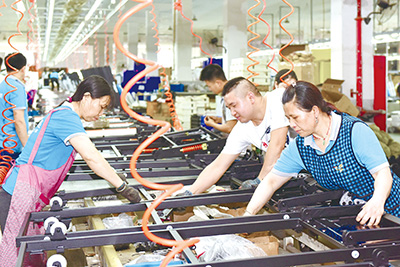
\includegraphics[width=123.528000mm,trim=4.973874mm 0.000000mm 4.973874mm 0.000000mm,clip]{./img_article/jh2_image1.jpeg}\par

\end{tcolorbox}
\end{mytcbox1}\end{staticcontents*}
\begin{staticcontents*}{statico5}\begin{mytcbox1}[width=\textwidth,height=0.394000\textheight]\begingroup
\setlength{\columnsep}{0pt}
\begin{wrapfigure}{r}{88.0pt}
\begin{tikzpicture}[scale=1]
%maintitle
\node[rectangle,text width =51.0pt] (a)
{\scalebox{1}[0.7554054054054055]{\syht{\bfseries\fontsize{51.0}{32}\selectfont \shortstack[c]{全\\国\\知\\名\\作\\家\\诗\\人\\再\\访\\艾\\青\\故\\里}\par}}};
%maintitle2\node[right=0pt of a,rectangle,text width =51.0pt] (b)
%maintitle2{\scalebox{1}[0.7554054054054055]{\syht{\bfseries\fontsize{51.0}{32}\selectfont \shortstack[c]{全国知名作家诗人再访艾青故里2}\par}}};
%%subtitle2
%righttitle\node[right =0pt of b,rectangle,text width =21pt]
%righttitle{\heiti{\bfseries\fontsize{21}{17}\selectfont \par}};
%%subtitle1
\node[left =0pt of a,rectangle,text width =21pt]
{\heiti{\bfseries\fontsize{21}{17}\selectfont 共赴诗歌盛宴 传承艾青精神\par}};
\end{tikzpicture}\par
\vspace{-\baselineskip}
\end{wrapfigure}
{\songti{\fontsize{9}{10}\selectfont \setlength{\parindent}{2em}本报讯(记者 季凯琳)昨日,来自全国各地的诗人、作家欢聚金义新区(金东区),参加为期3天的第三届艾青诗歌节之“我爱这土地”全国知名作家诗人艾青故乡行第二期活动。\par     今年是诗坛泰斗艾青诞辰110周年,也是我区迎接设区20周年的关键之年。今年7月23日至25日,我区成功举办第三届艾青诗歌节之“我爱这土地”全国知名作家诗人艾青故乡行第一次活动。为深化活动成果,提升“和美金东、希望新城”文化“金名片”影响力,我区举办了第二期活动。\par     本次活动由中国诗歌学会、北京大学中国诗歌研究院、区委宣传部主办,区文联、区文旅局协办,邀请了内蒙古、杭州、四川等多个省市作家协会副主席,《中国汉诗》《莽原》《扬子江》等多家杂志社的主编、副主编,还有中国对外文化集团艺术委员会委员、中国诗歌学会驻会副会长、上海大学教授等。\par     近年来,我区持续深化名人文化品牌聚力工程,深入推进“人文富区”战略,大力打造诗歌之城,不断为诗歌文化传承发展创设新路径、新载体,将诗歌文化植入城市发展,形成了一大批诗路旅游地,推动经济发展。\par     活动期间,作家诗人们将前往艾青文化公园、曹宅盆景长廊、曹宅镇雅里村、艾青故居、傅村镇中心小学、菜鸟网络金华园、孝顺镇麦磨滩文化产业园采风,深入了解20年里我区在新农村建设、城市建设和文化传承等方面的成果。之后,作家诗人们将参加礼堂乡村文化宴暨“星空下的诗会”,通过现场活动+网络云直播+两地互动(星空下的诗会和乡村诗会)+云游金东的形式,传诵艾青诗歌,弘扬艾青诗歌精神。\par 此外,8月29日下午举办的“城市发展与诗歌”主题研讨会也不容错过。诗人们将通过思想的碰撞交流,探讨城市发展与诗歌的有机融合,以诗人和作家的视角,共同为我区发展出谋划策。\par \par}}\par
\endgroup
\end{mytcbox1}\end{staticcontents*}
\begin{staticcontents*}{statico6}\begin{mytcbox1}[width=\textwidth,height=0.436000\textheight]\begin{center}
%%subtitle1
{\heiti{\fontsize{21}{0}\selectfont \par}}
\vspace{0mm}
%maintitle
{\scalebox{0.6431893687707642}[1]{\syht{\fontsize{43}{0}\selectfont \shortstack[c]{江岭高新智造区“\\微小区”激发新动能}\par}}}\par
%%subtitle2
\vspace{0mm}
{\heiti{\fontsize{21}{0}\selectfont }}\par
\vspace{5mm}
\end{center}
{\songti{\fontsize{9}{10}\selectfont \setlength{\parindent}{2em}本报讯(记者 盛瀚潇)8月24日晚8时,江岭高新智造区党群服务中心内灯火通明,附近企业职工三五成群走出宿舍,携家带口来到服务中心休闲娱乐,看看电影,逛逛夜市,别提多热闹了。\par     融休闲、娱乐、体验于一体的党群服务中心成了员工们的好去处。有了烟火气,原本清冷的园区道路变成了热闹的集市小广场。“以前一下班就待在宿舍玩手机,放假就想回老家,现在服务中心娱乐项目多,比老家还舒服,我们很喜欢这里的生活。”浙江好易点公司外来员工杨峰说。\par     坐落在江东镇的江岭高新智造区是区级重点工业园区,经过8年的开发建设,目前已落户企业280家,吸引就业人员逾万人。企业人员密集,娱乐消费和生活服务需求旺盛,但园区地处城郊,周边商业配套资源薄弱,影响了企业职工队伍的稳定性。“园区周边除了公司就是工厂,我们下班也没地方去。”浙江迈腾工贸有限公司员工付业勇说。\par     “如何聚群力、惠企业,让配套服务符合职工所盼所想,这些是我们重点考虑的问题。”区高新智造产业集群党建联盟党委书记李志阳表示,今年,依托新建成投入使用的党群服务中心开拓消费市场,丰富园区配套设施,设置了咖啡吧、电影吧、读书吧、中介服务等场所。同时通过招引各类平台资源,为企业职工提供品牌饮品、书籍租赁、金融服务、岗位招聘等生活服务。\par     考虑到服务中心场地有限,不能完全满足员工消费需求,党群服务中心拓宽本地线下配送渠道,依托江东果蔬基地等平台,以“范围配送+党员代跑”模式把生活品送到员工手中。\par “稳企发展,留人是关键,江岭高新智造园区打造小区式配套服务,既方便企业员工,又贴心服务,让员工找到了归属感,增强他们对岗位的依附度。”区委组织部副部长、区委两新工委书记方晓辉表示,未来,金义新区(金东区)将通过全面完善党群服务中心服务功能来提升企业集聚区的生活配套,让“党建红”为打造营商生态最优区而建,兼具企业职工视觉和感觉属性,用最优最暖的服务,集聚最优人才。\par \par}}\par\vspace{3.000000mm}

\includegraphics[width=87.120000mm,height=33.210000mm]{./bh_image/1.png}\par
\end{mytcbox1}\end{staticcontents*}


\end{document}